\section{Optimization}
\label{sec:optimization}

The performance of the inference algorithm implementation on GraphX highly
depends on how we partition the graph. A good partitioning strategy should be
able to evenly distribute the vertices to each partition so that no partition
is so large that it is hard to be computed or stored.  In this section, we
first present a partitioning strategy, tailored towards message-passing style
inference algorithms on message passing graphs, to achieve the goal of a good
partitioning strategy.

Next, we present a way of optimizing shuffling in GraphX. The optimization
eliminates the majority of shuffle in InferSpark. The optimization involves a
complete re-write of GraphX, but it keeps all the API of GraphX so the porting
of InferSpark from GraphX to the optimized version is effortless.

\subsection{Discussion on Partitioning Strategies}

\begin{figure}[h]
	\includegraphics[width=0.45\textwidth]{figs/mixture_mpg.eps}
	\caption{Message Passing Graph of a Mixture Model}
	\label{fig:mixture_mpg}
\end{figure}

GraphX adopts a vertex-cut partitioning approach.
The vertices are replicated in edge partitions instead of edges being replicated in vertex
partitions. 
The four built-in partition
strategies in GraphX are: 
EdgePartition1D (1D),
EdgePartition2D  (2D),
RandomVertexCut (RVC), and
CanonicalRandomVertexCut (CRVC).
In the following, we first show that these general 
partitioning strategies perform badly for the VMP algorithm on MPG.
\KZ{Does it only perform badly on VMP? What about Gibbs and EP?}
Then, we introduce our own partitioning strategy.

\figref{fig:mixture_mpg} shows a more typical message passing graph of a
mixture model instead of the toy two-coin model that we have used so far. $N$
is the number of $x$ and $z$, $K$ is the number of $\phi$, $D$ is the number
of $\theta$. Typically, $N$ is very large because that is the data size (e.g.,
number of words in LDA), $K$ is a small constant (e.g., number of topics in
LDA), and $D$ could be a constant or as large as $N$ (e.g., number of
documents in LDA). 


EdgePartition1D essentially is a random partitioning strategy, except that it
co-locates all the edges with the same source vertex. Suppose all the edges from
$\phi_k$ are assigned to partition $k$. Since there's an edge from $\phi_k$ to
each one of the $N$ vertices $x$, partition $k$ will have the replications
of all $x_1, x_2, \ldots, x_N$. In the best case, 
edges from different $\phi_k$ are assigned to different
partitions. Then the largest edge partition still have at least $N$ vertices.
When $N$ is very large, the largest edge partition is also very large, which
will easily cause the size of an edge partition to exceed the RDD block size limit. However,
the best case turns out to be the worst case 
when it comes to the number of vertex replications
because it actually replicates the size $N$ data $K$ times, which is
extremely space inefficient. The over-replication also incurs large amount of
shuffling when we perform outer joins because each updated vertex has to
be shipped to every edge partition, prolonging the running time. 

We give a more formal analysis of the number of vertices in the largest edge
partition and the expected number of replications of $x_i$ under
EdgePartition1D. As discussed above, there's at least one edge partition that
has replications of all the $x_i$'s. 
Observe that the graph has an upper bound of
$3N + K$ vertices, so the number of vertices in the largest edge partition is
$O(N)$. Let $N_{x_i}$ be the number of replications of $x_i$, then the expected
number of replication of $x_i$ is 
\begin{align*}
	E[N_{x_i}] &= M(1 - (1 - \frac{1}{M})^{K+1}) \\
		&= \left\{
			\begin{array}{ll}
				(K + 1) + o(1) & K = O(1) \\
				M + o(1) & K = O(M) 
			\end{array}
		\right.%}
\end{align*}



%first introduction 
%then analysis
\begin{figure}[h]
	\centering
	\includegraphics[scale=0.25]{figs/2dhash.eps}
	\caption{EdgePartition2D. Each grid is a partition. 
	The possible partitions where $x_i$ is
	replicated is shaded}
	\label{fig:2dhash}
\end{figure}

EdgePartition2D evenly divides the adjacency matrix of the graph into $\sqrt{M}
\times \sqrt{M}$ partitions. The vertices are uniformly distributed along the
edges of the adjacency matrix by hashing into $\sqrt{M}$ buckets. The upper
bound of the number of replications of a vertex $x_i$ is $\sqrt{M}$ because all
the edges that point to it are distributed to at most $\sqrt{M}$ partitions
in shown as \figref{fig:2dhash}.  Meanwhile, there are $K+1$
edges pointing to $x_i$, so the number of replications of $x_i$ cannot exceed
$K+1$ as well. Therefore, the upper bound of replications of $x_i$ is actually
$\min(K+1, \sqrt{M})$. On the other hand, suppose each of the $\phi_k$ is
hashed to different bucket and $N$ $x$'s are evenly distributed into the
$\sqrt{M}$ buckets, then the number of largest partition is at least
$\frac{N}{\sqrt{M}}$, which is still huge when the average number of words per
partition is fixed. Following is the formal analysis of the EdgePartition2D.

Let $B$ be an arbitrary
partition in the dark column on \figref{fig:2dhash}.
Let $Y_{x_i, B}$ be the indicator variable for the event that $x_i$ is replicated in 
Then the expectation of $Y_{x_i, B}$ is
\begin{align*}
	E[Y_{x_i, B}] &= 1 - (1 - \frac{1}{\sqrt{M}})^{K+1} \\
\end{align*}

The number of vertices $N_B$ in the largest partition $B$ is at least the expectation
of the number of vertices in a partition, which is also at least the
expectation of the number of $x_i$ in it:
\begin{align*}
	E[N_{B}] &= \sum_{v} E[Y_{v, B}] \\
		&\ge \frac{N}{\sqrt{M}} E[Y_{x_i, B}]	\\
		& = \left\{
				\begin{array}{ll}
					(K + 1)\eta	+ o(1) & K = O(1) \\
					\sqrt{M}\eta + o(1) & K = O(M) 
				\end{array}
			\right.%}
\end{align*}

The expected number of replications of $x_i$ is
\begin{align*}
	E[N_{x_i}] &= \sqrt{M}E[Y_{x_i, B}] \\
		&= \left\{
			\begin{array}{ll}
				(K + 1) + o(1) & K = O(1) \\
				\sqrt{M} + o(1) & K = O(M) 
			\end{array}
		\right.%}
\end{align*}


%
RandomVertexCut (RVC) uniformly assigns each edge to one of the $M$
partitions. The expected number of replications of $x_i$ tends to be $O(K)$
when $K$ is a constant and tends to be $O(N)$ when $K$ is proportional to the
number of partitions. The number of vertices in the largest partition is also
excessively large. It is $O(K\frac{N}{M})$ when K is a constant and $O(N)$
when $K$ is proportional to the number of partitions.  CanonicalRandomVertexCut
assigns two edges between the same pair of vertices with opposite directions
to the same partition. For VMP, it is the same as RandomVertexCut since only
the destination end of an edge is replicated. For example, if $x_i$ has $K +1$
incoming edges, then the probability that $x_i$ will be replicated in a
particular partition is independent from whether edges in opposite
direction are in the same partition or randomly distributed. Therefore 
CRVC will have the same result as RVC.  
\tabref{tab:max_v_per_edge_part_O1} and
\tabref{tab:max_v_per_edge_part_OM} summarize the comparison of different
partition strategies.

InferSpark's partitioning strategy is actually tailor-made for VMP's message passing graph.
The intuition is that the MPG has a special structure.
For example, in \figref{fig:mixture_mpg},
we see that the MPG essentially has $D$ ``independent'' trees rooted at $\theta_i$,
where the leaf nodes  are $x$'s and they form a complete bipartite graph with all $\phi$'s.
In this case, one good partitioning strategy is to form $D$ partitions, 
with each tree going to one partition and the $\phi$'s getting replicated $D$ times.
We can see that such a partition strategy incurs no replication on $\theta$, $z$, and $x$,
and incurs $D$ replications on $\theta$.

Generally, our partitioning works as follows: Given an edge, we first determine
which two random variables (e.g. $x$ and $z$) are connected by the edge. It is
quite straightforward because we assign ID to the set of vertices of the same
random variable to a consecutive interval. We only need to look up which
interval it is in and what the interval corresponds to. Then we compare the
total number of vertices correponding to the two random variables and choose
the larger one. Let the Vertex ID range of the larger one to be $L$ to $H$. We
divide the range from $L$ to $H$ into $M$ subranges. The first subrange is $L$
to $L + \frac{H-L+1}{M}$; the second is $L + \frac{H-L+1}{M} + 1$ to $L +
2\frac{H-L+1}{M}$ and so on. If the vertex ID of the edge's chosen vertex falls
into the $m^{th}$ subrange, the edge is assigned to partition $m$.

In the mixture case, at least one end of every edge is $z$ or $x$. Since
the number of $z$'s and $x$'s are the same, 
each set of edges that link to the $z_i$ or $x_i$ with 
the same $i$ are co-located. This guarantees that $z_i$
and $x_i$ only appears in one partition. All the $\phi_k$'s are replicated in each
of the $M$ partitions as before. The only problem is that many $\theta_j$ with
small $N_j$ could be replicated to the same location. In the worst case, the
number of $\theta$ in one single partition is exactly $\eta$. However, it is
not an issue in that case because the number of vertices in the largest
partition is still a constant $3\eta + K$. It is also independent from whether $K
= O(1)$ or $K = O(M)$.


\begin{table}[h]
	\centering
	\caption{Analysis of Different Partition Strategies When $K = O(1)$}
	\label{tab:max_v_per_edge_part_O1}
	\small
	\begin{tabular}{lll}
		\hline
		Partition Strategy & $E[N_{x_i}]$ & $E[N_B]$\\\hline\hline
		1D & $O(K)$ & $O(N)$ \\\hline
		2D & $O(K)$ & $O(K\frac{N}{M})$ \\\hline
		RVC & $O(K)$ & $O(K\frac{N}{M})$ \\\hline
		CRVC & $O(K)$ & $O(K\frac{N}{M})$ \\\hline
		{\bf InferSpark} & 1 & $3\frac{N}{M}+1$ \\\hline
	\end{tabular}
\end{table}

\begin{table}[h]
	\centering
	\caption{Analysis of Different Partition Strategies When $K = O(M)$}
	\label{tab:max_v_per_edge_part_OM}
	\small
	\begin{tabular}{lll}
		\hline
		Partition Strategy & $E[N_{x_i}]$ & $E[N_B]$\\\hline\hline
		1D & $O(M)$ & $O(N)$ \\\hline
		2D & $O(\sqrt{M})$ & $O(\sqrt{M}\frac{N}{M})$ \\\hline
		RVC & $O(M)$ & $O(N)$ \\\hline
		CRVC & $O(M)$ & $O(N)$ \\\hline
		{\bf InferSpark} & 1 & $3\frac{N}{M}+1$ \\\hline
	\end{tabular}
\end{table}

\subsection{Optimizing Shuffle}
\label{sec:optimize_shuffle}

Data shuffle is an expensive operation in a distributed system because it
involves a lot of random disk I/Os and large amount of network traffic between each
pair of workers. In the case of Apache Spark, either slow random disk I/O or
low network bandwidth is a bottleneck of the shuffle performance. In most
cases, the random I/O is the main contributing factor to the poor shuffle
performance although shuffle file consolidation mitigates the problem
\cite{spark-shuffle}.

The way that GraphX implements data shuffle is to simply re-partition the
vertices or messages according to the partitioner of the RDD to be zip-joined
with uses. GraphX first flat maps each vertex partition $i$ to an array of
vertex blocks. The vertices in block $j$ are the vertices that need to be
replicated in edge partition $j$.  Block $j$ is also paired with the partition
ID $j$ so that it can be re-partitioned using the edge RDD's partitioner.
Finally, GraphX calls ``partitionBy'' on the resulting RDD to get an RDD of
replicated vertices that is zip-joinable with the edge RDD.

Under our partitioning strategy, there is one single edge partition to which
most of the vertices are replicated, for each of the vertex partitions. The
shuffle size will be greatly reduced if these vertices are not actually
shuffled to the edge partitions.

\begin{figure}
	\centering
	\includegraphics[scale=0.5,clip]{figs/graph_partition.eps}
	\caption{Design of a graph partition}
	\label{fig:inferspark_graph_partition}
\end{figure}

The solution is to merge the vertex partition with the edge partition to which
most of the vertices are replicated into a single partition (see
\figref{fig:inferspark_graph_partition}).  The replicated vertices in such a
partition reduces to those were not in the vertex partition before the merge.
Therefore, we only need to shuffle those vertices that were not in the
corresponding vertex partition before merge in order to complete the
replication. In the case of InferSpark, most vertices are referenced from only
one edge partition. Thus the optimization eliminates almost all the shuffle
during vertex replication.

The change in the implementation does not necessarily break the GraphX API
since we can still provide a Vertex RDD view and an Edge RDD view via
projection. Hence, porting InferSpark to the optimized GraphX is effortless.

\subsection{Handling Intermediate RDDs}

Both the original GraphX and the optimized version persist some intermediate
RDDs behind the scene for performance consideration, making it hard for the
generated inference code to properly unpersist all the unnecessary cached
RDDs. For example, the underlying RDD of GraphX prior to vertex replication is
hidden when the vertex replication occurs. It will be persisted if the graph
is persisted prior to vertex replication, wasting the precious memory of
executors.

We modified GraphX to keep track of the intermediate RDDs so that they are
unpersisted whenever an action is invoked on the final RDD. With this feature,
we can avoid persisted RDDs being accumulated in the cache.


